\chapter{Methodology}
\label{chap:methodology}

This chapter describes the proposed data analytics workflow to detect and
localize events in computer networks through end-to-end measurements. Also, the
QoS data gathering procedures are briefly presented. Finally, the proposed
system is compared with previous projects.

\section{Measurement Process}

The time series used in this work represent network end-to-end measures of a
cable-television infrastructure, which runs DOCSIS with asymmetric download and
upload bandwidths. Home routers connected to cable modems communicate
with servers strategically located by the ISP\@. Each server is responsible
for measurements of several end-users.
Measurements are triggered in
each home router in every half hour and, by the end of every day,
the results are transferred to a database.
The software responsible for these procedures was
developed by TGR (a startup at COPPE/UFRJ),
and is spread over approximately four thousand customers of a major Brazilian
Tier-3 ISP\@.

To measure the round
trip packet loss fraction and the RTT between the home router and the associated
server, the
home router sends a train of short UDP packets, and the server bounces back
them. The data here presented considers a train of 100 UDP packets of 32 bytes,
separated by 1 millisecond.
Also, the traceroutes from the end-users
to the respective servers are collected with the same frequency. Traceroutes
from servers to end-users are not gathered.
In~\cite{a_preliminary_performance_measurement_study_of_residential_broadband_services_in_brazil},
a preliminary descriptive investigation of loss fraction, RTT and other metrics
is presented.

The resulted time series are unevenly spaced due to a range of reasons. First,
measurements are initiated only if the residential link is not under use by the
ISP customer. Also, the client may have no Internet connection to start a
measurement, or even be without electrical energy.

\section{Pipeline}

This section describes, in a high level abstraction, the proposed workflow
used to detect network events and localize their cause. When necessary, some
steps are better explored in further sections.
The analysis seeks for events during a specific time period, in a single
measurement server, and considers a
single metric (loss fraction or RTT), which are specified as parameters.
Therefore, a complete analysis can be accomplished considering different
executions with distinct parameters.
Figure~\ref{fig:pipeline} illustrates the process.

\begin{figure}[H]
    \centering
    \includegraphics[width=0.9\linewidth]{./figures/methodology/pipeline/pipeline.png}
    \caption{Pipeline.}
\label{fig:pipeline}
\end{figure}%

The workflow starts with the End-Users Filtering step,
which aims to remove clients that can negatively affect the analysis.
As an example, this work eliminates clients
that don't have enough measurements, or present
traceroute inconsistencies (in Section~\ref{sec:spatial_correlation}
this issue is better examined).

The Change Point Detection phase preprocess the end-users time series and
identify change points.
Also, the change points are classified in three types of events: failure,
improvement, or inconclusive. For both QoS metrics used,
a change point defines a
failure event if the average of the window after this point is greater than the
average of the window before. The improvement event is analogous, however is
characterized by a mean decrease.
The inconclusive event means that the segments averages are too close.

The Spatial Correlation procedure cluster the end-users in end-groups
according with their position in the network. This clustering can then be used
in further steps to isolate possible events locations.
This stage must produce a specific grouping structure, which is detailed in
Section~\ref{sec:spatial_correlation}.

The Events Times Correlation aims to combine similar events of different
end-users of an end-group. For example, if three end-users detect a failure at
the same time, then this information will be identified in this step.
The clustered end-users events are named as network events.
The details of this method are enlightened in
Section~\ref{sec:events_times_correlation}.

Finally, to localize the events cause, the Spatial-Time Correlation
matches network events
from different user-groups with the end-groups structure.
This is better explained in Section~\ref{sec:spatial_time_correlation}.

\section{Spatial Correlation}
\label{sec:spatial_correlation}

This procedure enables to check which network equipments are shared by end-users
that perceive the same network event. The used strategy was guided by the
specific ISP's topology.

The server position relative to the end-user
can be categorized in two contexts.
In the OFF-NET case, the traffic between them
goes through a Tier-2 ISP\@.
However, in the ON-NET case, the traffic
doesn't leave the Tier-3 ISP infrastructure.
The latter situation represents a simpler IP topology, since the Tier-3 ISP
uses static routing and
doesn't applies load balancing nor MPLS, techniques that are usual in the Tier-2
ISP network.

Therefore, considering measurements against a single server and the ON-NET
case, paths from end-users to the server form a hierarchically
structured topology, which is a required design to be consumed by the
Spatial Time Correlation procedure~\ref{sec:spatial_time_correlation}.
It is
This work doesn't have access to the ISP network
topology, therefore, this structure is reconstructed through traceroutes.
In this context, each equipment that responds to traceroutes
pings are used as user-groups.

The first hop of the traceroutes, which corresponds to the home gateway, is
removed from the analysis. Also, CMTSs are reported with their private IPs,
since they are in the same subnetwork of the end-users.
Therefore, to differentiate distinct CMTSs, the
user-groups are defined by their reported IP and the first public IP that
appears from their hop until reach the server. Additionally, not all CMTSs are
configured to answer to traceroute pings.

In the OFF-NET case, due to the load balancing applied by the Tier-2 ISP,
the traceroute reconstruction doesn't lead in a hierarchical topology.
To overcome this issue, sequential hops related to the
the Tier-2 ISP are compressed to a single hop.
As an example, the path (Tier-3 Router 1, Tier-2 Router 1, Tier-2 Router 2,
Tier-3 Router 2, Server) is
transformed to (Tier-3 Router 1, Tier-2, Tier-3 Router 2, Server).
In general, this process conducts to a hierarchical topology,
the exception happens when the Tier-2 ISP has output connections to
different routers of the Tier-3 ISP in the same network region.
However, this is an uncommom situation in
the current dataset, and then was removed from the analysis.
The distinction between
Tier-3 and Tier-2 hops is made thorough the investigation of hops names.

Figure~\ref{fig:real_graph} presents an example of the reconstructed
topology. The routers were anonymised. The ``Tier-2'' and ``Server''
user-groups are self explanatory. The others are represented by a tuple, in
which the first field indicates the reported IP in the traceroute, and the
second specifies the first hop until reach the server that reported a public
IP\@.

\begin{figure}[H]
    \centering
    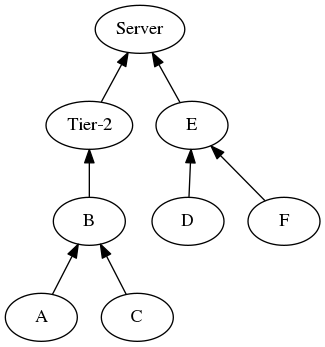
\includegraphics[width=\linewidth]{./figures/methodology/spatial_correlation/dtstart2016-05-01_dtend2016-05-11_NRIDTCLDM031_graph_anonymized.png}
    \caption{User-groups topology.}
\label{fig:real_graph}
\end{figure}%

During the End-Users Filtering step, some clients are removed due to traceroute
inconsistencies~\cite{avoiding_traceroute_anomalies_with_paris_traceroute}.
As an example, the same equipment can appear in different hops. Also,
considering that the software limits the maximum number of hops, it were
removed the cases in which the traceroute didn't reach the server.
Since routing tables can be updated, it were only considered clients
in which the traceroute didn't change during the specified time period.

\section{Events Times Correlation}
\label{sec:events_times_correlation}

The motivation of this step is to, given the change points of each end-user of
an end-group, infer network events that can explain these end-users events.

There are two main reasons to detect the same network event, such as an
equipment failure, at different times in different clients. The first one is
related to the fact that the time series are not regularly sampled. The second
one is due to the change point detection algorithm behavior.
Therefore, a procedure to group end-users events based on their type and time,
should be flexible enough to take into consideration time delay effects. Also,
it must be robust to deal with multiple change points per time series.

In order to relax a change point location, a detected change point is
transformed into an interval in accordance to a time tolerance.
Therefore, given a parameter $\delta$, a change point identified at
time $t$ means that exists a change point within
$[t - \delta, t + \delta]$. To be consistent,
change point algorithms must report locations separated by more than
$2 \delta$ time units. The algorithms presented in
Chapter~\ref{chap:change_point_detection}
can be easily adapted to respect this restriction. However, this can also be
achieved by the following post processing step:
sweeping time from left to right, if two
points are at most $2 \delta$ time units apart, then the right one is removed.

Then, the problem can be defined as selecting a set of network events,
that explain all end-users events of a end-group.
An end-user event is explained by a network event if they have the same type,
and the end-user event time is inside the network event time interval.
This problem has several possible solutions, and the comparison between
them is subjective. As an example, not
necessarily selecting the minimum number of network events that cover all
end-user events is the most appropriate answer.
Also, considering a specific event type, it is required that network events
time intervals have an empty intersection.

To this goal, it was developed a heuristic inspired in the inexact voting in
totally
ordered space~\cite{voting_algorithms} problem. In this problem, people
vote in a single point in the real line, and also considering a $\delta$
parameter, the objective is to
select the interval with the biggest number of voters.

The created greedy procedure, called here as Multiple Inexact Voting in Totally
Ordered Space, is specified in
Algorithm~\ref{alg:multiple_inexact_voting_totally_ordered_space}

\begin{algorithm}[H]
\caption{Multiple Inexact Voting in Totally Ordered Space}
\label{alg:multiple_inexact_voting_totally_ordered_space}
    \begin{algorithmic}[1]
        \State{Let $l$ be the end-users events of a specific type sorted by
        time}
        \While{$l$ is not empty}
            \State{Select the interval $d$ with the biggest number of
            end-users events,
            in which all these events are at most $2 \delta$ apart.
            In case of ties select the left most one}
            \State{Report the mean time of
            the $d$ extremes as the network event time}
            \State{Remove all end-users events from $l$ that are in $d$}
        \EndWhile{}
    \end{algorithmic}
\end{algorithm}

It is possible to note that, in each iteration the procedure solves an instance
of the inexact voting in totally ordered space.

A more straighforward solution, that was not used in this work, is to create
regular time-bins, and interpret all end-users events that occur at the same
bin as a common network event.
However, this strategy can introduce
discontinuities. If a network event occur in the end/beginning of a time-bin,
then it is likely to different end-user events associated with this
network event be located in different bins.

If co-occurrent events with the same type affect the same user-group,
it is not possible to distinguish them. Nonetheless, the probability of
detecting different events at the same time can reduce with the increase
of the time series sampling frequency.

\section{Spatial-Time Correlation}
\label{sec:spatial_time_correlation}

PROBLEM OF TWO WAY METRICs.

These step aims to correlate network events detected in different user-groups
to localize network events.

Suppose a single network event, defined by a time and a type. The following
analysis is based in the inclusion/exclusion principle. Also, it considers that
if a specific equipment presents a failure or an improvement, all QoS metrics
in which the traffic goes through this equipment will sense the modification.
Also, it is considered that if a change point detection setup is able to
detect a network event in a end-user dataset, it will also be able to detect
the same event in other end-user time series if this event impacted both
end-users. Also it is considered that co-occurrent events are not possible.

Suppose that only a proper subset of the clients of an user-group defined by a
leaf in the user-group topolgy detects the event. Therefore, through the
suppositions is possible to afirm that these clients share some common network
equipment before the first hop that caused the event. It is possible to exclude
the first or posterior hops from this conclusion, since not all clients which
traffic goes to this first hop detected the event.

However if a all clietns of the first hop detected the event, then the  problem
can be this hop. But also can be before the first hop if all clients share a
single equipment before the hop. Also can be after the first hop. To check the
after, the same kind of analysis is applied to the next hop to the server. If
not all clients of the second hop detected this event, then the problem is not
at the second hop. So for sure is at most at the first hop. However if all
clients of the second hop have the problem than then analysis recursively goes
untill reach a case of find a hop without every clients with the event or
reaching the server.

This analysis is made for every possible path to the server, that is, starting
for each leaf of the user-group topology.

However different paths share common network equipments and the resulted
problematic components gathered from each path analysis can be correlated. The
list of possible problematic locations from a path analysis consists of a path
prefix from the end-user to the server. If in different path the same network
event is detected, then they must share at least one equipment in commum. The
ones that are not in commom can be discarded from the problematic list, since
there are other clients that don't passes through them and present the problem.
It is possible to note that this commom problems will be a suffix mathc of this
prefix problems.

Figure~\ref{fig:network_events_locations_examples} presentes several topologies
and different network events. The gray vertexes indicate a real network event
that occurre in this location.

\begin{figure}[H]
    \centering
    \makebox[\textwidth][c]{%
        \begin{subfigure}[b]{0.2\textwidth}
            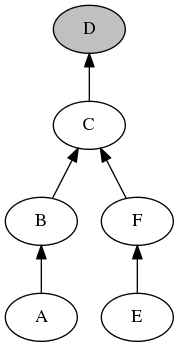
\includegraphics[width=\textwidth]{./figures/methodology/spatial_time_correlation/event_tree_graph_1.png}
            \caption{}\label{fig:network_events_locations_examples_1}
        \end{subfigure}
        \begin{subfigure}[b]{0.2\textwidth}
            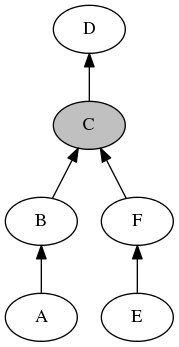
\includegraphics[width=\textwidth]{./figures/methodology/spatial_time_correlation/event_tree_graph_2.png}
            \caption{}\label{fig:network_events_locations_examples_2}
        \end{subfigure}%
        \begin{subfigure}[b]{0.3\textwidth}
            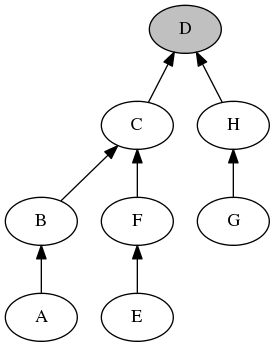
\includegraphics[width=\textwidth]{./figures/methodology/spatial_time_correlation/event_tree_graph_3.png}
            \caption{}\label{fig:network_events_locations_examples_3}
        \end{subfigure}
        \begin{subfigure}[b]{0.3\textwidth}
            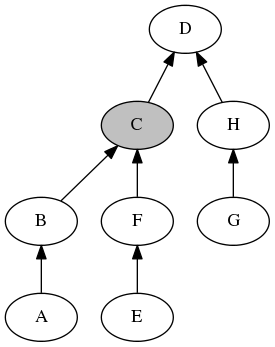
\includegraphics[width=\textwidth]{./figures/methodology/spatial_time_correlation/event_tree_graph_4.png}
            \caption{}\label{fig:network_events_locations_examples_4}
        \end{subfigure}%
    }
    \caption{Network events locations examples.}
\label{fig:network_events_locations_examples}
\end{figure}%

In Figure~\ref{fig:network_events_locations_examples_1} the analysis made
in the path (A, B, C, D) result in the following possible events locations (A,
B, C, D). The analysis made in the path (E, F, C, D) results in the following
possible locations (E, F, C, D). Correlating both paths results checking the
suffix of the prefix, the possible locations are (C, D). In
Figure~\ref{fig:network_events_locations_examples_2} the analysis is the same
of the previous case.

In Figure~\ref{fig:network_events_locations_examples_3} the analyis made in the
all paths result in the own path. Correlating the resultings the output is the
D vertex.

In Figure~\ref{fig:network_events_locations_examples_4} the analysis in path
(G, H, D) don't detect the event. The path (A, B, C, D) find that (A, B, C) are
the possible locations. Path (E, F, C, D) result in the (E, F, C) possible
locations. Correlating the results of different paths result in the C vertex,
which is exacly the correct location.

The comparison of network events of different user-groups is made comparing if
they are close enough.

If more than one network event of the same type occur at the same type is
possible to have an empty suffix match if the some affected end-users don't
share components. Threfore, to avoid this situation, the analysis only
considers paths that share the last problematic vertex.

Also the tree topolgy requirement can be relaxed, and the a similar algorithm
can be derived in cases where there is only load balancing per source address.
However since this case is not applied in the current dataset, this extension
is not presented in this dissertation.

As will be seen in Chapter~\ref{chap:conclusions} this kind of analysis suffer
from sparsiness of the clients, for example several vertex can be traversed by
the same clients.

\section{Change Point Detection Issues}

As stated in Chapter~\ref{chap:change_point_detection}, one of the main issues
of this work is the algorithms and parameters selection.
In general, this process requires a dataset to enable the evaluation of an
algorithm setup.

There are several approaches to construct a
change points dataset in the literature.
Some works create simulated time series, in which distinct segments are sampled
by the same generative model with different
parameters~\cite{change_point_detection_in_time_series_data_by_relative_density_ratio_estimation}.
In general, this type of data is more easily handled by change point detection
algorithms, since some methods assume the same models used in the dataset
building process. Also, real data can have complex characteristics that are
difficult to be reproduced by generative models. Another strategy is to join
segments from different real time series with different
characteristics~\cite{inertial_hidden_markov_models_modeling_change_in_multivariate_time_series}.
However, this can introduce unreal change points scenarios. Since one of
the goals of this work is to deal directly with real data,
this approach was discarded.

When the latent information of the time series are available, and if there is a
complete knowledge of what configurations changes in the latent state impact
data, it is possible to check the change points only analyzing this underlying
information. As an example, consider a time series that represents the cardiac
frequency of a soccer player during a match. Also, consider that in this
controlled environment, the only causes of changes in the cardiac frequency are
the variations of physical activities, such as starting or stopping to run.
Therefore,
it is possible to use the times in which a player changed his movement behavior
as the change points, whithout even analyzing the time series. However, in the
application domain of the present work, this approach would be impractical.
First, this would need the expertise of how the configurations of network
topology, routers congestion, physical equipment problems, among other features,
affect the different end-to-end QoS metrics.
Second, this kind of information is absent in the dataset, and would be too
complex to collect it.

Another way is to use visual annotations,
as it was done
in~\cite{learning_sparse_penalties_for_change_point_detection_using_max_margin_interval_regression}.
Also, manual labeling is usual for anomaly indentification in traffic
traces~\cite{webclass_adding_rigor_to_manual_labeling_of_traffic_anomalies}.
In this strategy, an application domain expert is exposed to a time series,
and visually indicates his opinion about the change points locations.

It is known that visual inspection methods can bring erroneous
conclusions~\cite{leveraging_cloud_data_to_mitigate_user_experience_from_breaking_bad},
and also amplify subjectivity, however, to better understand the problem, this
approach was experimented in this work.

Through a web system a user freely marked the change points with a mouse.
The fact that data is not regularly sampled in time could bring an unwanted
visual change perception. Therefore, the X axis of the displayed time series
represented only the temporal order of the measures.
It was only presented raw
loss fraction time series with 10 days of data.
Also, it was selected only the ones that have at
least 85\% of the maximum possible number of points during the specified period,
considering that data is sampled at most two times in a hour. Change points can
be interpreted as rare events in this dataset, and several data streams have
almost
all measures with zero losses. Therefore, to increase the entropy,
it was only selected time series that have at least one window of length 48 with
more than 5 measures with loss fraction larger than 0.01.

Additionally, it was provided a set of tips to the specialist:

\begin{itemize}
    \item In the case of packet loss fraction, mean changes between 0 and 0.1
    are more sensible to the end users.
    \item The time axis only represents the temporal order of the measurements.
    However, in general, consecutive points in time axis are separated by 30
    minutes.
    \item Outlier is not a statistical change. An outlier is an observation that
    lies outside the overall pattern of a distribution.
\end{itemize}

Figure~\ref{fig:survey_system} presents a system's snapshot.
The vertical red line means that the user marked a change point in that
position.

\begin{figure}[H]
    \centering
    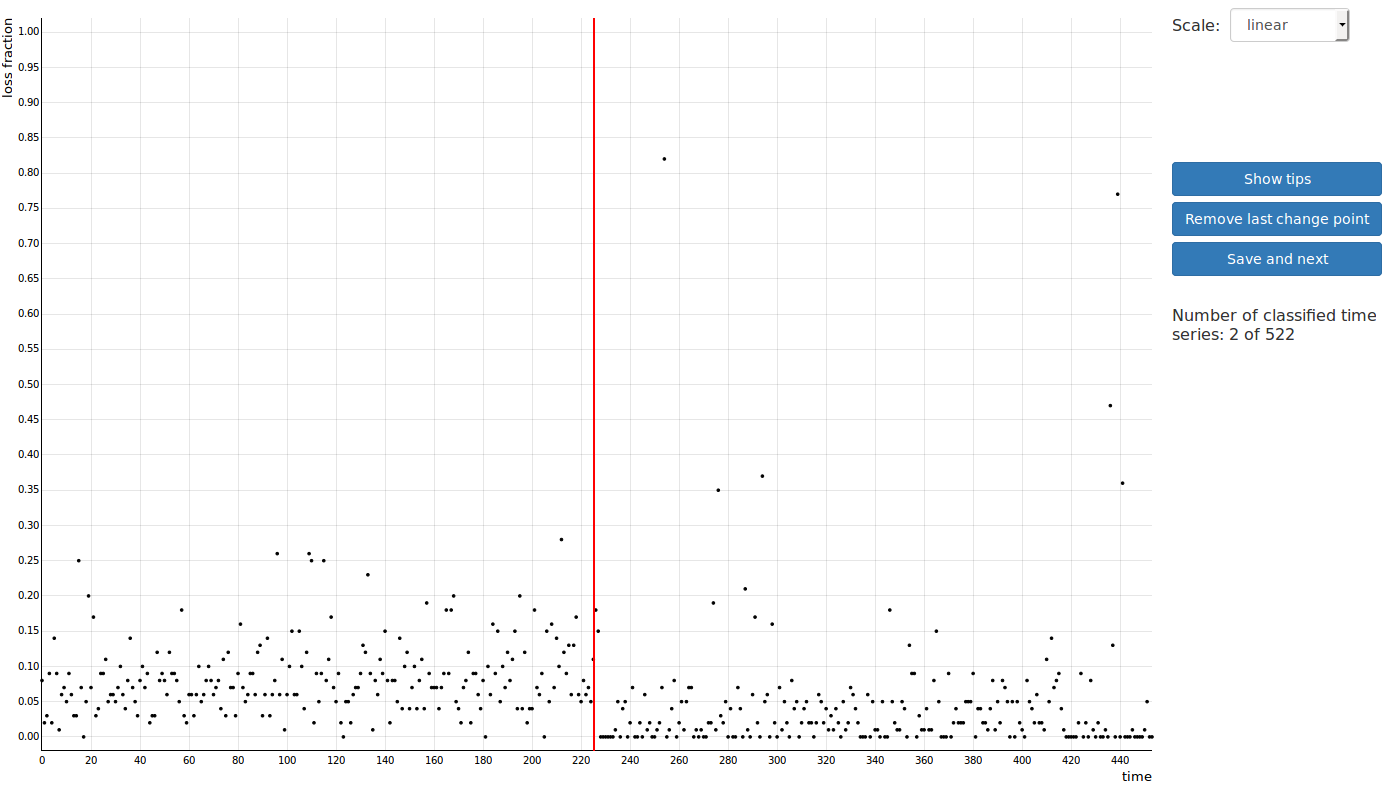
\includegraphics[width=0.9\linewidth]{./figures/methodology/supervised_learning_try/survey_system.png}
    \caption{Survey system snapshot.}
\label{fig:survey_system}
\end{figure}%

Six specialists with experience in network measurements and statistical
modeling, but without background in change point detection, classified 71 time
series.
To analyze the agreement between different users classifications,
for each time series, was applied the Events Times Correlation procedure
described in Section~\ref{sec:events_times_correlation}. Therefore, it was
considered that each specialist voted to a set of change points positions.
The time tolerance was set to 7 hours, which means 14 consecutive points.

Then, for each change point voted at least once, it was counted the number of
specialists that voted in that location.
Figure~\ref{fig:classifications_per_vote} shows the histogram of this counting.

\begin{figure}[H]
    \centering
    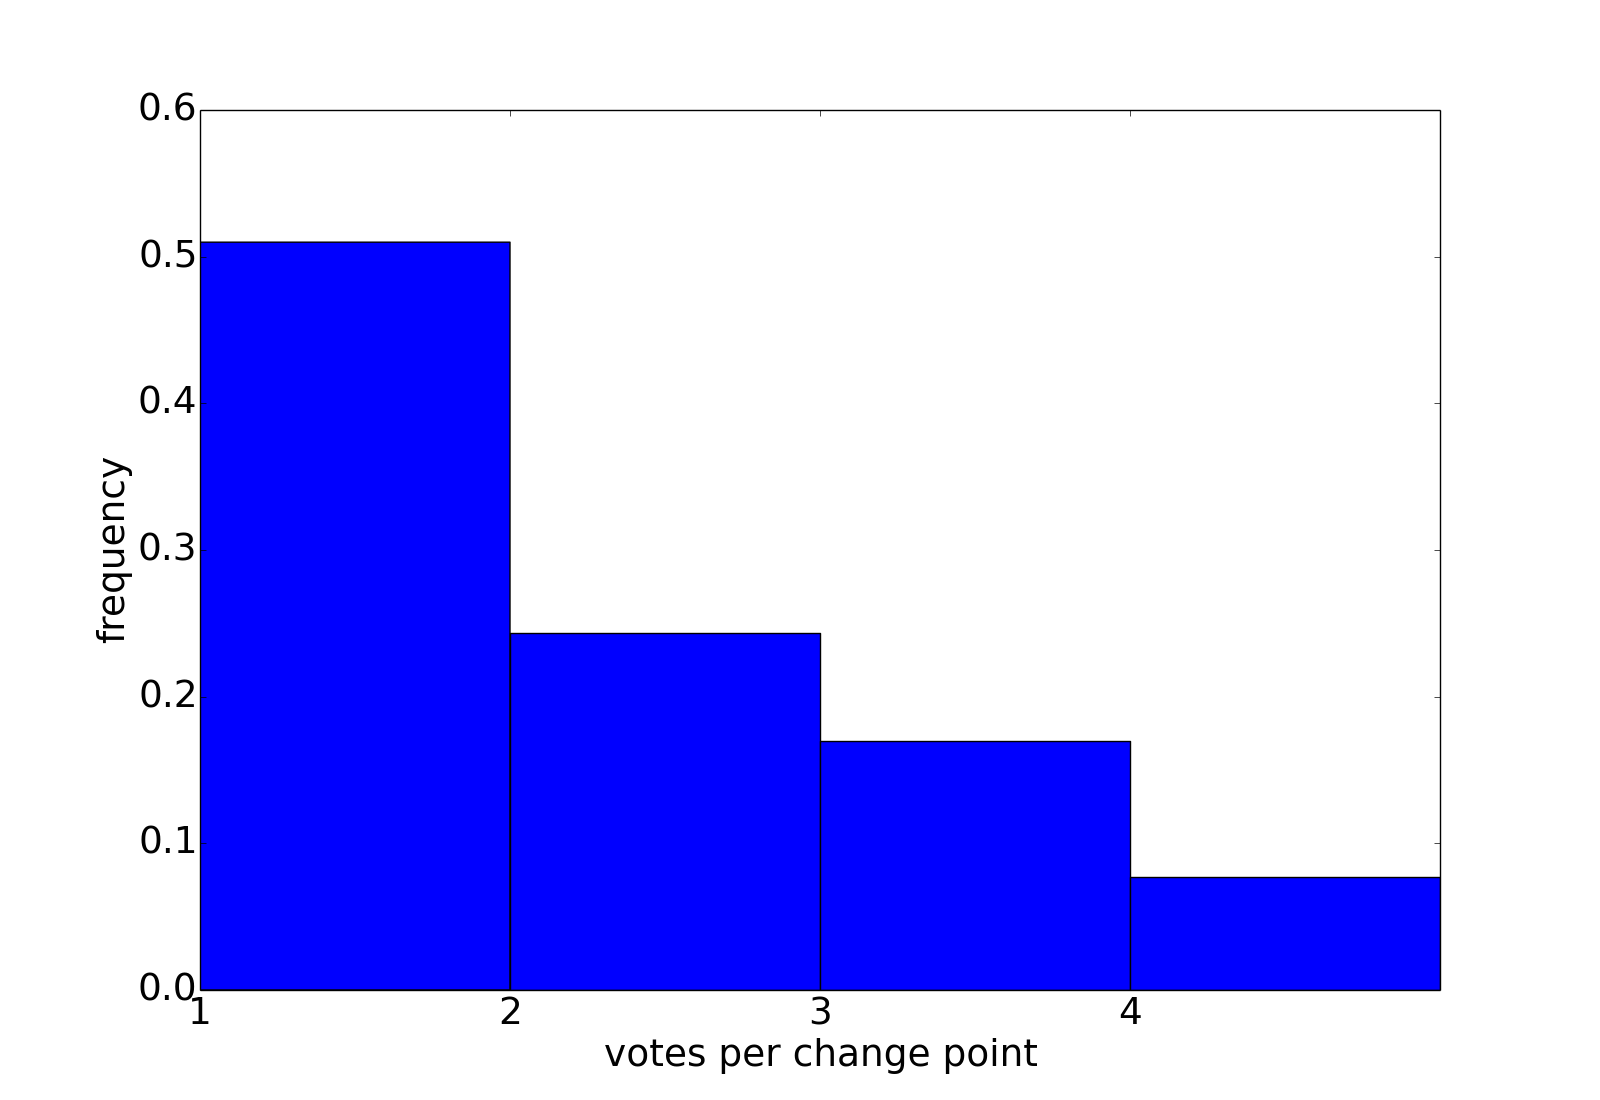
\includegraphics[width=0.7\linewidth]{./figures/methodology/supervised_learning_try/cnt_classifications_per_vote.png}
    \caption{Number of votes per change point histogram.}
\label{fig:classifications_per_vote}
\end{figure}%

It is possible to note that, 44\% of the change points were only voted by
a single user, and only 23\% were voted by the majority (more than 3 votes).
Therefore, in general, the consensus of change point locations is low.

In Figure~\ref{fig:classification_match} is presented the specialists
classifications in a time series with a high level of agreement on the change
points locations.
However, Figure~\ref{fig:classification_mismatch} shows a time series with
several disagreements.
It was verified that the latter case is the most representative in the
constructed dataset, fact that corroborates the problem subjectiveness.

\begin{figure}[H]
    \centering
    \makebox[\textwidth][c]{%
        \begin{subfigure}[b]{0.55\textwidth}
            \includegraphics[width=\textwidth]{{./figures/methodology/supervised_learning_try/cnt6_serverNHODTCSRV04_mac64:66:B3:A6:BC:B8_dtstart2016-05-01_dtend2016-05-11/rosam@land.ufrj.br}.png}
            \caption{Specialist 1}\label{fig:classification_match_1}
        \end{subfigure}
        \begin{subfigure}[b]{0.55\textwidth}
            \includegraphics[width=\textwidth]{{./figures/methodology/supervised_learning_try/cnt6_serverNHODTCSRV04_mac64:66:B3:A6:BC:B8_dtstart2016-05-01_dtend2016-05-11/gustavo.santos@tgr.net.br}.png}
            \caption{Specialist 2}\label{fig:classification_match_2}
        \end{subfigure}
    }
    \makebox[\textwidth][c]{%
        \begin{subfigure}[b]{0.55\textwidth}
            \includegraphics[width=\textwidth]{{./figures/methodology/supervised_learning_try/cnt6_serverNHODTCSRV04_mac64:66:B3:A6:BC:B8_dtstart2016-05-01_dtend2016-05-11/guisenges@land.ufrj.br}.png}
            \caption{Specialist 3}\label{fig:classification_match_3}
        \end{subfigure}
        \begin{subfigure}[b]{0.55\textwidth}
            \includegraphics[width=\textwidth]{{./figures/methodology/supervised_learning_try/cnt6_serverNHODTCSRV04_mac64:66:B3:A6:BC:B8_dtstart2016-05-01_dtend2016-05-11/gabriel.mendonca@tgr.net.br}.png}
            \caption{Specialist 4}\label{fig:classification_match_4}
        \end{subfigure}
    }
    \makebox[\textwidth][c]{%
        \begin{subfigure}[b]{0.55\textwidth}
            \includegraphics[width=\textwidth]{{./figures/methodology/supervised_learning_try/cnt6_serverNHODTCSRV04_mac64:66:B3:A6:BC:B8_dtstart2016-05-01_dtend2016-05-11/edmundosilva@gmail.com}.png}
            \caption{Specialist 5}\label{fig:classification_match_5}
        \end{subfigure}
        \begin{subfigure}[b]{0.55\textwidth}
            \includegraphics[width=\textwidth]{{./figures/methodology/supervised_learning_try/cnt6_serverNHODTCSRV04_mac64:66:B3:A6:BC:B8_dtstart2016-05-01_dtend2016-05-11/edmundo@land.ufrj.br}.png}
            \caption{Specialist 6}\label{fig:classification_match_6}
        \end{subfigure}
    }
    \caption{Classifications agreements.}
\label{fig:classification_match}
\end{figure}%

\begin{figure}[H]
    \centering
    \makebox[\textwidth][c]{%
        \begin{subfigure}[b]{0.55\textwidth}
            \includegraphics[width=\textwidth]{{./figures/methodology/supervised_learning_try/cnt6_serverCTBDTCLDM91_mac64:66:B3:A6:B7:BC_dtstart2016-05-01_dtend2016-05-11/rosam@land.ufrj.br}.png}
            \caption{Specialist 1}\label{fig:classification_mismatch_1}
        \end{subfigure}
        \begin{subfigure}[b]{0.55\textwidth}
            \includegraphics[width=\textwidth]{{./figures/methodology/supervised_learning_try/cnt6_serverCTBDTCLDM91_mac64:66:B3:A6:B7:BC_dtstart2016-05-01_dtend2016-05-11/gustavo.santos@tgr.net.br}.png}
            \caption{Specialist 2}\label{fig:classification_mismatch_2}
        \end{subfigure}
    }
    \makebox[\textwidth][c]{%
        \begin{subfigure}[b]{0.55\textwidth}
            \includegraphics[width=\textwidth]{{./figures/methodology/supervised_learning_try/cnt6_serverCTBDTCLDM91_mac64:66:B3:A6:B7:BC_dtstart2016-05-01_dtend2016-05-11/guisenges@land.ufrj.br}.png}
            \caption{Specialist 3}\label{fig:classification_mismatch_3}
        \end{subfigure}
        \begin{subfigure}[b]{0.55\textwidth}
            \includegraphics[width=\textwidth]{{./figures/methodology/supervised_learning_try/cnt6_serverCTBDTCLDM91_mac64:66:B3:A6:B7:BC_dtstart2016-05-01_dtend2016-05-11/gabriel.mendonca@tgr.net.br}.png}
            \caption{Specialist 4}\label{fig:classification_mismatch_4}
        \end{subfigure}
    }
    \makebox[\textwidth][c]{%
        \begin{subfigure}[b]{0.55\textwidth}
            \includegraphics[width=\textwidth]{{./figures/methodology/supervised_learning_try/cnt6_serverCTBDTCLDM91_mac64:66:B3:A6:B7:BC_dtstart2016-05-01_dtend2016-05-11/edmundosilva@gmail.com}.png}
            \caption{Specialist 5}\label{fig:classification_mismatch_5}
        \end{subfigure}
        \begin{subfigure}[b]{0.55\textwidth}
            \includegraphics[width=\textwidth]{{./figures/methodology/supervised_learning_try/cnt6_serverCTBDTCLDM91_mac64:66:B3:A6:B7:BC_dtstart2016-05-01_dtend2016-05-11/edmundo@land.ufrj.br}.png}
            \caption{Specialist 6}\label{fig:classification_mismatch_6}
        \end{subfigure}
    }
    \caption{Classifications disagreements.}
\label{fig:classification_mismatch}
\end{figure}%

Also, it is possible to note that some users apparently changed their
classification pattern in the same time series. As an example,
Figure~\ref{fig:diff_class_same_time_series} presents two specialists that fits
this description. Also, in general, users changed their classification pattern
in different time series.

\begin{figure}[H]
    \centering
    \makebox[\textwidth][c]{%
        \begin{subfigure}[b]{0.55\textwidth}
            \includegraphics[width=\textwidth]{{./figures/methodology/supervised_learning_try/cnt6_serverNHODTCSRV04_mac64:66:B3:A6:B6:36_dtstart2016-05-01_dtend2016-05-11/rosam@land.ufrj.br}.png}
            \caption{Specialist 1}\label{fig:diff_class_same_time_series_1}
        \end{subfigure}
        \begin{subfigure}[b]{0.55\textwidth}
            \includegraphics[width=\textwidth]{{./figures/methodology/supervised_learning_try/cnt6_serverNHODTCSRV04_mac64:66:B3:A6:B6:36_dtstart2016-05-01_dtend2016-05-11/edmundo@land.ufrj.br}.png}
            \caption{Specialist 6}\label{fig:diff_class_same_time_series_6}
        \end{subfigure}
    }
    \caption{Different classification pattern in the same time series.}
\label{fig:diff_class_same_time_series}
\end{figure}%

Since this initial experiment resulted in a noisy dataset, in which change
points probably don't reflect real network events, this strategy was aborted.
Also, it would difficult to scale the study to include more
specialists and time series.

It is important to note that the algorithms described in
Chapter~\ref{chap:change_point_detection} are unsupervised methods.
Once a change point dataset is constructed, it is possible to apply supervised
learning procedures, which are not much explored in the change
point detection literature.

\section{Differences to Previous Systems}

The proposed data analytics architecture has several similarities with the
projects described in Chapter~\ref{chap:literature_review}.

As with Argus and NetNorad, this work clusters end-users in user-groups, however
with finer topology granularity. Also, to increase the system's scalability,
NetNorad and Argus use this grouping to reduce the number of tracked time
series. This strategy was not applied in this project,
since the finer granularity requires more time series to be spread in different
network locations, and the current dataset has a low number of end-users.

To detect faults, Argus applies an anomaly detection procedure, but the present
work uses a change point detection method. The difference between
these two problems is subtle, and can be fuzzy in the literature. The
anomaly detection assumes that a standard pattern is already known or
is identified by the procedure, then the goal is to find when the data
stream
deviates from it's standard. The change point detection only seeks for
points where the statistical properties change, and doesn't take into
consideration a standard time series behaviour.

Additionally, beyond the network edge point of view, Argus and NetNorad
uses some internal network information, which is absent in the present work.
